\documentclass[10pt,a4paper,notitlepage]{article}
\usepackage[utf8]{inputenc}
\usepackage{amsmath}
\usepackage{amsfonts}
\usepackage{amssymb}
\usepackage{graphicx}
\title{Crosstalk measurements from PAPER-64}
\author{Saul A. Kohn\thanks{saulkohn@sas.upenn.edu}\,\,\,\& James E. Aguirre\thanks{jeaguirre@sas.upenn.edu}\\ \small{University of Pennsylvania} }
\begin{document}
\maketitle

\abstract{XXX Crosstalk is artificial signal created by an interferometer that contaminates the visibilities.  In this memo, we describe measurements of crosstalk in data from PAPER-64. We present extremely compelling evidence that the dominant source of crosstalk for PAPER is reflections between antenna pairs, demonstrating a $1/R^2$ dependence for antenna-separation $R$. Some crosstalk is seen in excess of this trend, and may be due to crosstalk between dipole arms on individual antennae.}

\section{Introduction \& Theory}

XXX brief introduction and definitions\\
XXX do I even include D-terms?

\subsection{Reflection crosstalk}
We can describe crosstalk from reflections between antenna pair ($m,n$) as:
\begin{equation}
X'_m = X_m + \epsilon^x_{mn}X_n + \epsilon^y_{mn}Y_n;~~~~\epsilon^p_{mn}\propto\frac{1}{|m-n|^2}
\end{equation}
\noindent with a similar definition for $Y_m$. $|m-n|^2$ represents the physical distance between antennae $m$ and $n$.

This means that the observed $XX$ visibility between antennae becomes:
\begin{equation}
X'_mX'_n = X_mX_n + \epsilon^x_{nm}X_mX_m + \epsilon^x_{mn}X_nX_n + \epsilon^y_{nm}X_mY_m + \epsilon^y_{mn}Y_nX_n + \mathcal{O}(\epsilon^2)
\end{equation}
\noindent However the $XY$ visibilities are noise-like, so effectively:
\begin{equation}
X'_mX'_n \approx X_mX_n + \epsilon^x_{nm}X_mX_m + \epsilon^x_{mn}X_nX_n 
\end{equation}
\noindent Implying that the observed $XX$ visibilities are contaminated by over-the-air crosstalk from autocorrelations of nearby antennae.

\subsection{Dipole-arm crosstalk}
Crosstalk between dipole arms on a given antenna $m$ can be described by (neglecting noise terms):
\begin{align*}
X'_m = X_m + D^x_mY_m\\
Y'_m = Y_m + D^y_mX_m
\end{align*}
\noindent So an observed $XX$ visibility becomes contaminated by noise-like $XY$ and $YX$ visibilities:
\begin{equation}
X'_mX'_n = X_mX_n + D^x_mY_mX_n + D^x_nX_mY_n  + \mathcal{O}(D^2)
\end{equation}
\noindent Which is negligible compared to the $XX$ signal. However, this \textit{polarized leakage} is symmetric, causing $XX$ to leak into $XY$:
\begin{equation}
X'_mY'_n=X_mY_n + D^x_mY_mY_n + D^y_mX_nX_m + \mathcal{O}(D^2)
\end{equation}
\noindent This demonstrates the importance of trying to remove crosstalk when making measurements of polarization -- they will be completely overpowered by the $XX$ and $YY$ terms otherwise.

\section{Method}

We model crosstalk as if it is \textit{constant over time}. As shown above, this is not quite true, since the amount of reflection crosstalk is proportional to the autocorrelations, and these in turn are proportional to sky temperature. However, a constant over time is usually a good approximation, especially for the large amount of the season in which the Galaxy is not transiting zenith during observations.

Using this constant-over-time model, we proceed with a number of steps to constrain the crosstalk signal based on time-averaged visibilities, extracting the average visibility for each baseline:
\begin{itemize}
\item  over a 10 minute observation
\item  over a night of observations
\item  and for each baseline type over a night of observations
\end{itemize}
\noindent where ``baseline type" refers to a given antenna separation within the PAPER-64 grid. \textit{Crosstalk removal} is simply a subtraction of the nightly average for each baseline.

\section{Results}

In this section we will show the steps outlined in the section above, and our interpretation of... XXX\\

ALL FOR NIGHT 2456250\\


\begin{figure}
\centering
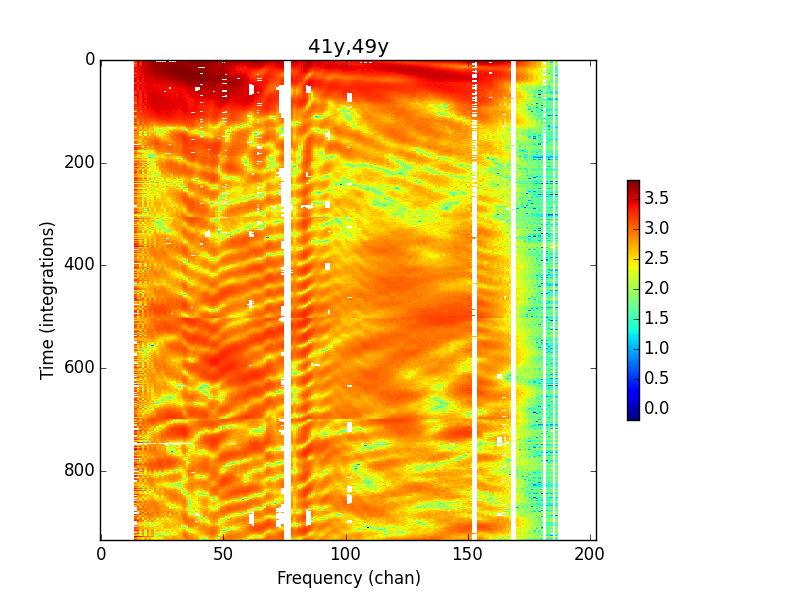
\includegraphics[width=0.4\textwidth]{6250_C.png}
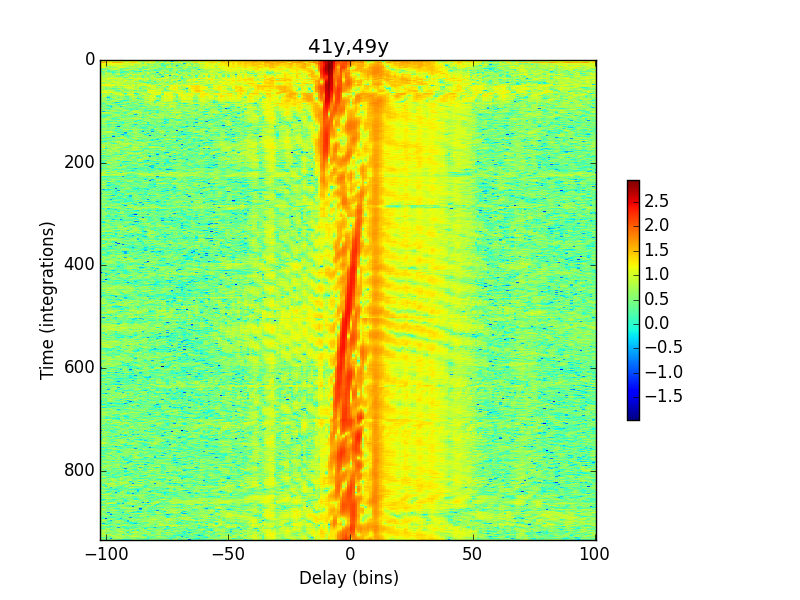
\includegraphics[width=0.4\textwidth]{6250_C_d.png}
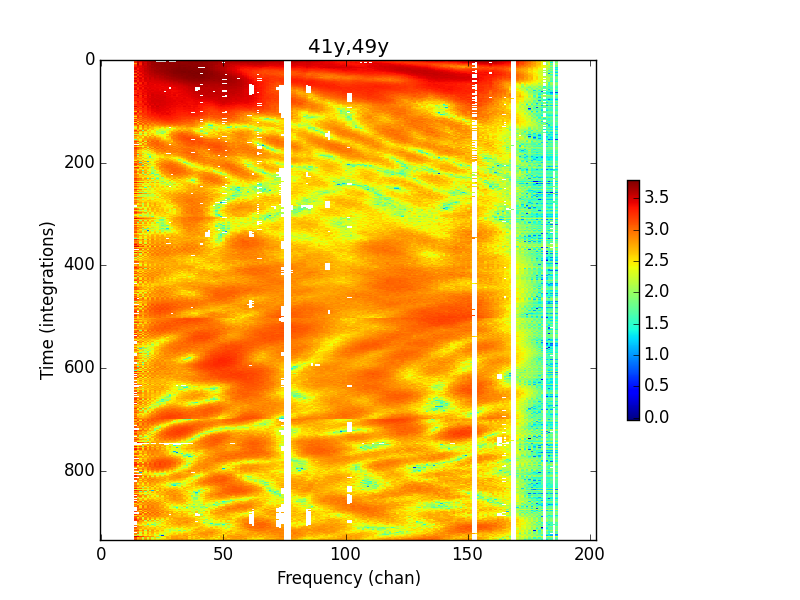
\includegraphics[width=0.4\textwidth]{6250_Cx.png}
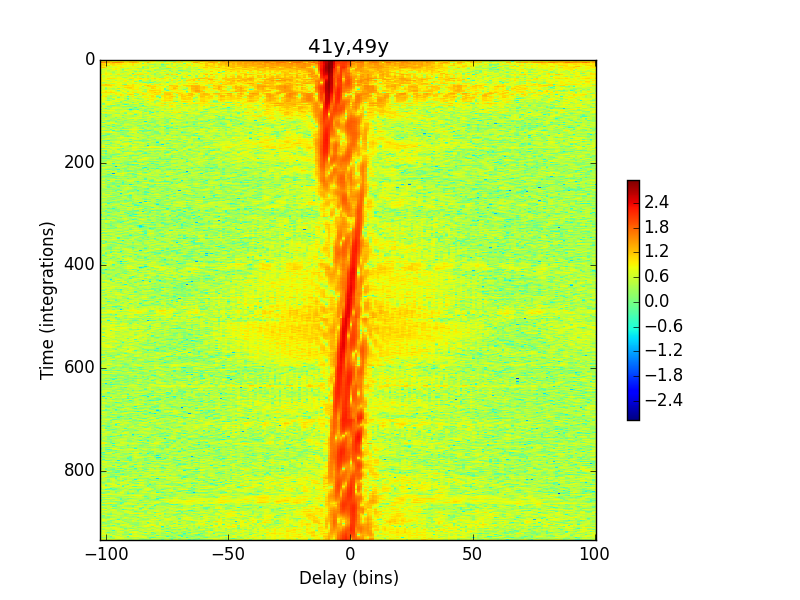
\includegraphics[width=0.4\textwidth]{6250_Cx_d.png}
\caption{\textit{Top}: Waterfall plots of the real part of $YY$ visibilities on a 30\,m baseline in frequency- (left) and delay-space (right). Note the constant-in-time signal on the horizon at positive delay. \textit{Bottom}: the same as above, but after crosstalk subtraction. The bright excess at integration numbers $<$200 is solar.}
\label{fig:waterfalls}
\end{figure}

\begin{figure}
\centering
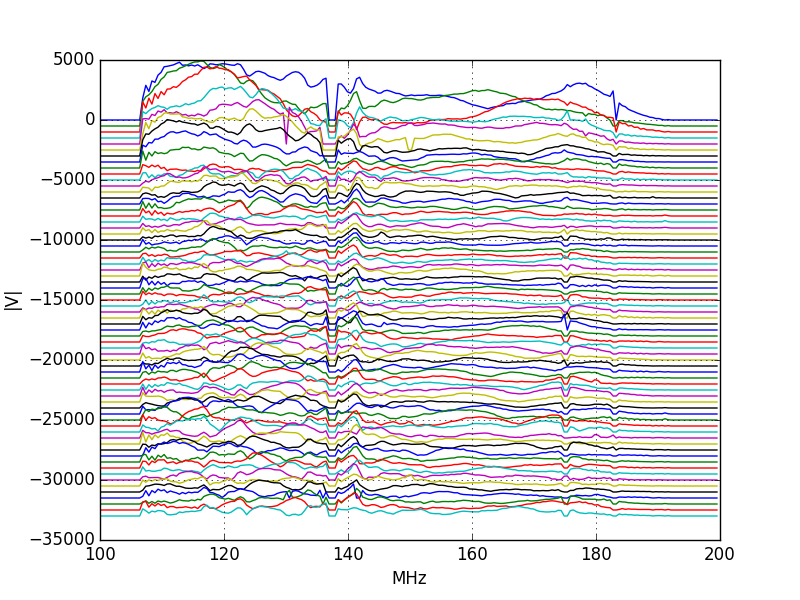
\includegraphics[width=0.4\textwidth]{6250_yy_xtalk_per_file.png}
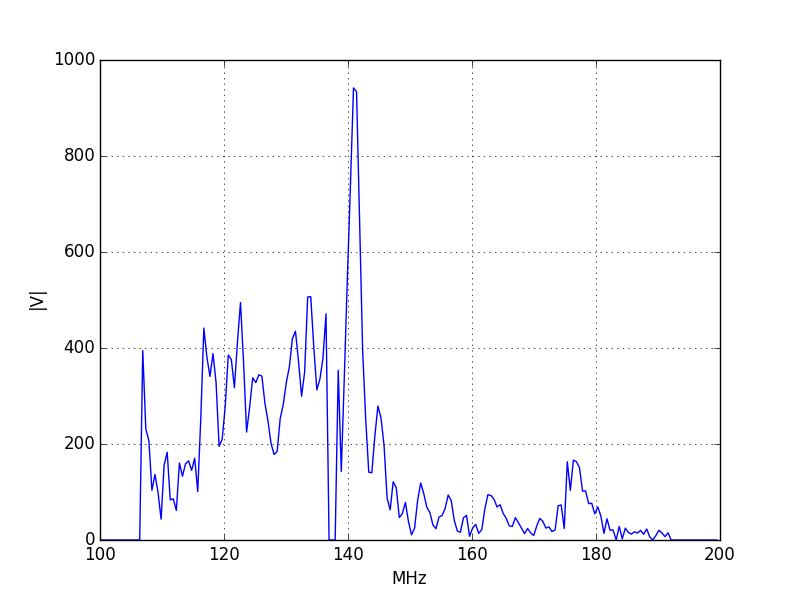
\includegraphics[width=0.4\textwidth]{6250_yy_xtalk_that_night.png}
\caption{\textit{Left}: The average $YY$ visibility for a 30\,m baseline of each 10 minute file over the night, plus a constant offset for display purposes. The average of the first file is at the top, and file time progresses downwards. \textit{Right}: The average of these signals (i.e. average for the night).}
\label{fig:xtalk-per-file}
\end{figure}

\begin{figure}
\centering
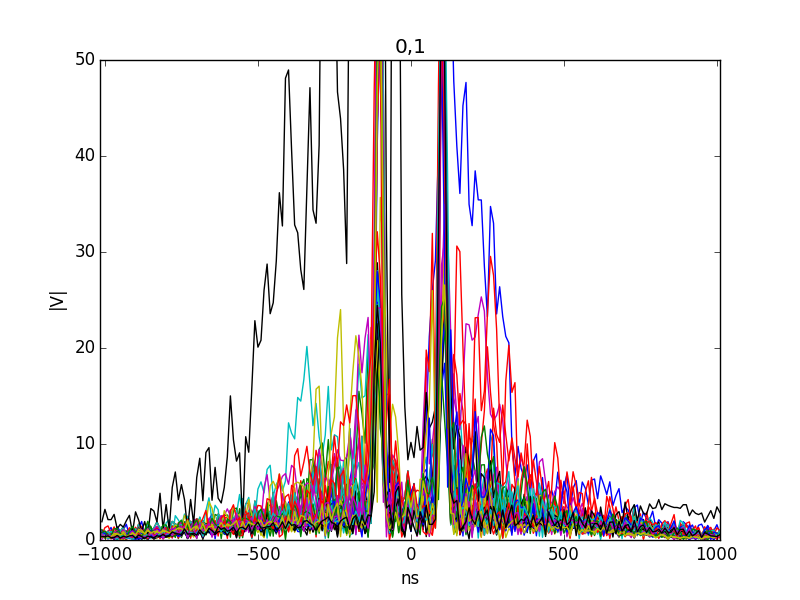
\includegraphics[width=0.4\textwidth]{6250_yy_xtalk_that_night_BLtype1_d.png}
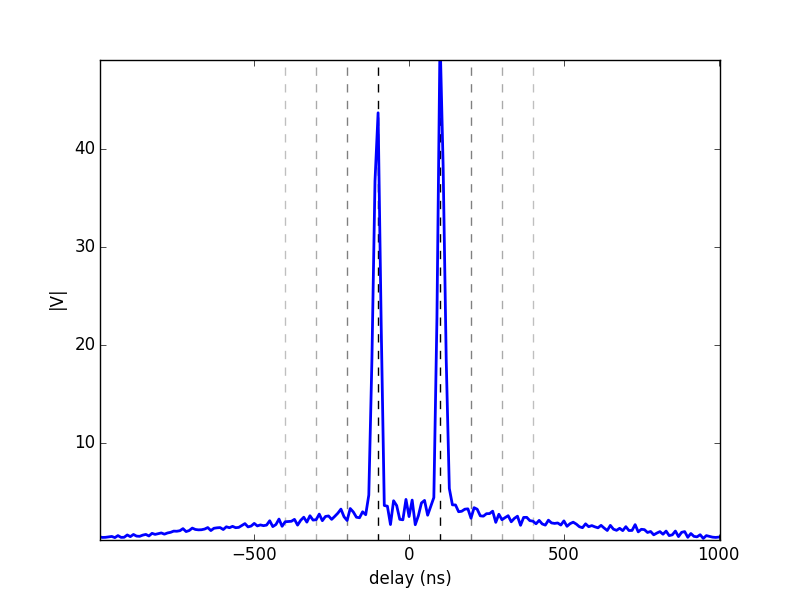
\includegraphics[width=0.4\textwidth]{6250_yy_xtalk_that_night_BLtype1_median_d.png}
\caption{\textit{Left}: The delay transform of the average signal for the night for all 30\,m baselines in the array. \textit{Right}: The average of these signals. The dotted lines show the light-travel-time between increasing grid separations (1, 2, 3 and 4-unit 30\,m baselines). There is a clear pile-up of signal at 1-unit delays.}
\label{fig:xtalk-for-BL1}
\end{figure}

\begin{figure}
\centering
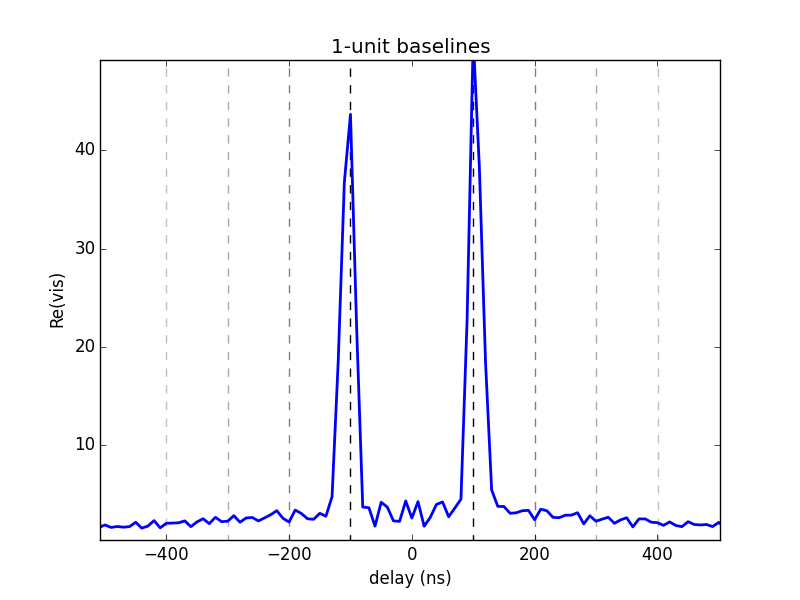
\includegraphics[width=0.4\textwidth]{xx_1unit_xtalk_d.png}
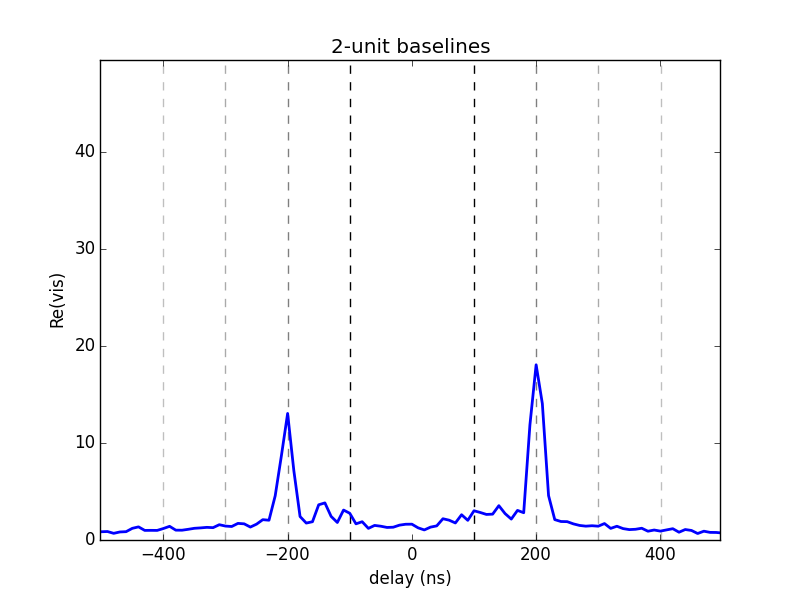
\includegraphics[width=0.4\textwidth]{xx_2unit_xtalk_d.png}
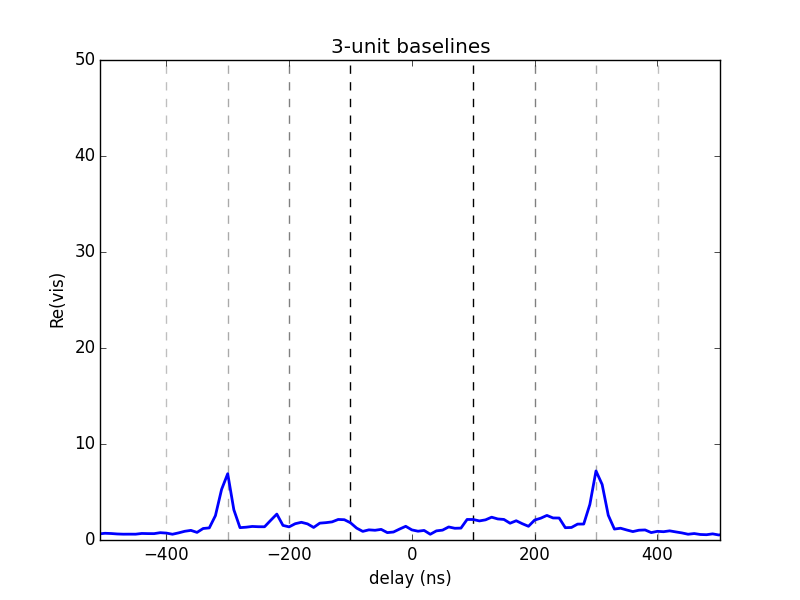
\includegraphics[width=0.4\textwidth]{xx_3unit_xtalk_d.png}
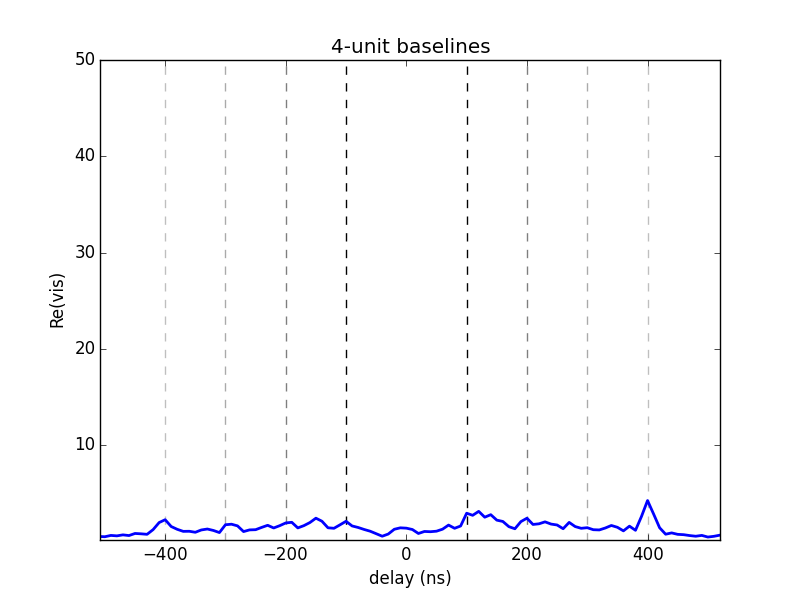
\includegraphics[width=0.4\textwidth]{xx_4unit_xtalk_d.png}
\caption{The average signal over the night in delay-space, averaged for baseline types of 30, 60, 90 and 120\,m separations.}
\label{fig:the-money-plot}
\end{figure}


\section{Conclusion}

\end{document}